\documentclass[11pt]{article}
\usepackage{graphicx}
\usepackage[bookmarks=true]{hyperref}
\usepackage{bookmark}
\usepackage{hyperref}
\usepackage{csquotes}
\usepackage{float}
\usepackage{wrapfig}
\usepackage{array}
\usepackage{wrapfig}
\newcolumntype{L}[1]{>{\raggedright\let\newline\\\arraybackslash\hspace{0pt}}m{#1}}
\newcolumntype{C}[1]{>{\centering\let\newline\\\arraybackslash\hspace{0pt}}m{#1}}
\newcolumntype{R}[1]{>{\raggedleft\let\newline\\\arraybackslash\hspace{0pt}}m{#1}}

\setlength{\parindent}{0pt}

\begin{document}
\begin{titlepage}
\begin{flushright}


\includegraphics[width=380px]{images/University_of_Pretoria_Logo.png}
\newline
\newline
\textbf {\LARGE Normalization Exercise - User Manual} \newline


\centering
\includegraphics[width=100px]{images/Logo.jpg}

\begin{flushleft}
\textbf {\Large Linphone for Andriod Group Chat (Waterfall)}\newline

\textbf {\Large Client: Nanoteq}\newline


\textbf {\large Version 1.0}\newline
\end{flushleft}
\centering \textbf {\large Authors:}

\begin{table}[H]
\large
\centering
\begin{tabular}{rl}
	Izak Blom & 13126777 \\
	David Breetzke & 12056503 \\
	Paul Engelke & 13093500 \\
	Prenolan Govender & 13102380 \\
	Jessica Lessev & 13049136 \\
\end{tabular}
\end{table}

Date: \today

\end{flushright}
\end{titlepage}

\setcounter{tocdepth}{3}
\setcounter{secnumdepth}{5}
\tableofcontents

\newpage
\section{Systems Overview}
The basis for this system is to provide a user with the ability to upload a chosen file of a certain extension. The system will then parse the file and return meta-data about the file such as file type. The system will then further parse the file and produce statistics regarding contents of the file. This includes the following statistics:
\begin{itemize}
\item Number of lines of code
\item Number of statements
\item Number of classes
\item Number of functions or methods
\item Average number of statements per class
\item Average number of statements per function
\item Lines of comments
\end{itemize}

\section{Systems Configuration}
The system is exported as a simple executable jar. A user can thus use any machine to run the application on.

\section{Installation}
No installation is necessary to make use of the application. The user simply needs to locate the executable file and double-click on it to open the application.

\section{Getting Started}
The user simply needs to locate the executable file and double-click on it to open the application.


\section{Using The System}
Below is a list of detailed steps on how to use the application.
\begin{enumerate}
\item Open the application\\
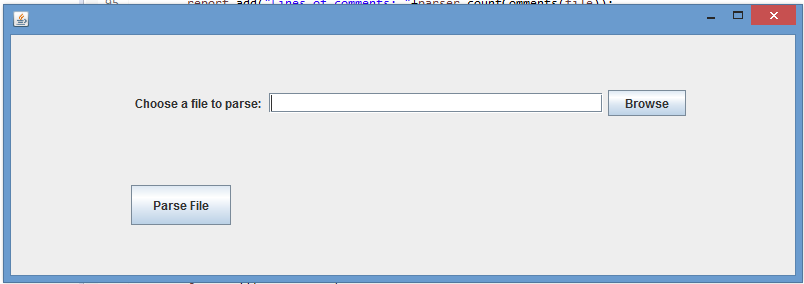
\includegraphics[width=100px]{images/home.png}
\item Click on "Browse" to upload a file\\
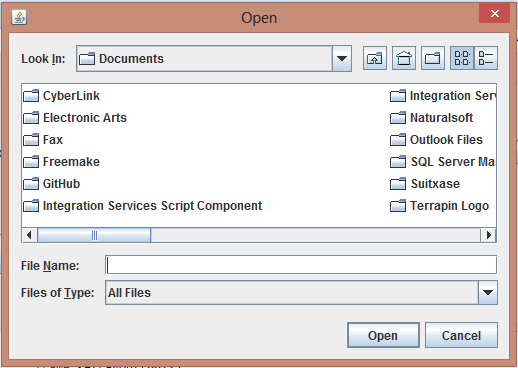
\includegraphics[width=100px]{images/browse.png}
\item Locate the desired file, select it and click "Open".\\
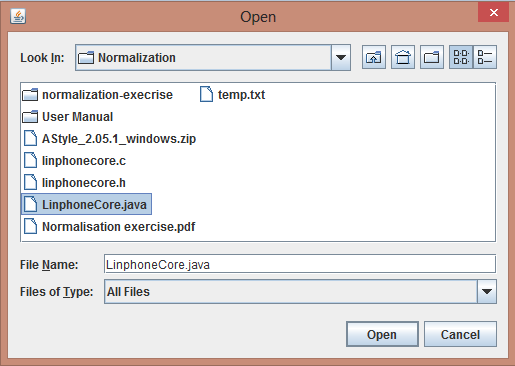
\includegraphics[width=100px]{images/select.png}
\item Click "Parse".\\
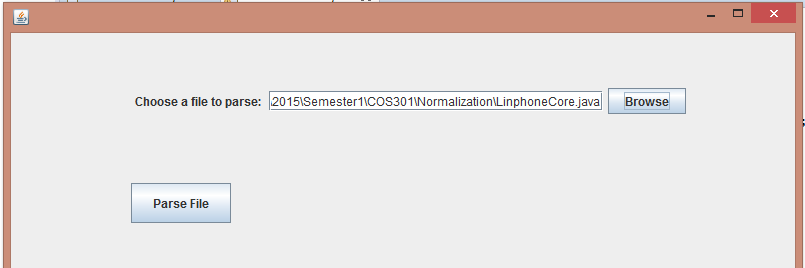
\includegraphics[width=100px]{images/parse.png}
\item Observe Results
\end{enumerate}


\section{Troubleshooting}
Below is a list of problems that may be encountered along with their possible solutions:
\subsection{Desired File not Located}
\textbf{Problem:} When "Browse" is clicked the desired file to be located is not found. \\
\textbf{Solution: } Search in all possible directories of computer to locate the file. Make sure that the file you are searching for exists. \\

\subsection{File not processed}
\textbf{Problem:} When "Parse" is clicked No results appear. \\
\textbf{Solution: } \begin{enumerate}
\item Make sure a file has been selected to be parsed.
\item Make sure the file that has been uploaded is supported by the application (C and Java).
\end{enumerate} 

\subsection{File incorrectly processed}
\textbf{Problem:} When "Parse" is clicked obviously wrong results appear. \\
\textbf{Solution: } \begin{enumerate}
\item Make sure the file that has been uploaded is supported by the application (C and Java).
\end{enumerate} 

\end{document}
